% Packages %%%%%%%%%%%%%%%%%%%%%%%%%%%%%%%%%%%%%%%%%%%%%%%%%%%
\documentclass[conference]{IEEEtran}
\IEEEoverridecommandlockouts 
\usepackage{cite}
\usepackage[cmex10]{amsmath}
\usepackage{amssymb}
%\usepackage{algorithmic}
\usepackage{array}
\usepackage{mdwmath}
\usepackage{mdwtab}
\usepackage{eqparbox}
\usepackage{graphicx}
\usepackage[]{subfigure}
\usepackage{url}
\usepackage[algoruled,vlined,linesnumbered]{algorithm2e}
\usepackage{verbatim}
\usepackage{color}
\usepackage{hyperref}
\usepackage{mathtools}

\makeindex 
\makeatletter

%%%%%%%%%%%%%%%%%%%%%%%%%%%%%%%%%%%%%%%%%%%%%%%%%%%%%%%%%%%%%%%%
% Magic stuff to shrink stuff
\makeatletter
\renewcommand\section{\@startsection{section}{1}{\z@}
                                  {-3.0ex plus -1.5ex minus -0.5ex}
                                  {0.7ex plus 1ex minus 0ex}
                                  {\bfseries}}
\renewcommand\subsection{\@startsection{subsection}{1}{\z@}
                                  {-2.0ex plus -1.5ex minus -0.5ex}
                                  {0.7ex plus 1ex minus 0ex}
                                  {\itshape\bfseries}}
\makeatother


%\newcommand{\shrinka}{\def\baselinestretch{0.99}\large\normalsize}

\long\def\IGNORE#1{}


%%%%%%%%%%%%%%%%%%%%%%%%%%%%%%%%%%%%%%%%%%%%%%%%%%%%%%%%%%%%
% Paper Info
\author{ Valerie Bazie $\quad\quad$ Carol Young $\quad\quad$ Ana Huam\'an Quispe%
	\thanks{The authors are with the Georgia Institute of
	Technology, Atlanta, GA 30332, USA. Email:
	{\tt\small vbazie3@gatech.edu},{\tt\small cyoung44@gatech.edu},
	{\tt\small ahuaman3@gatech.edu} }}
\title{ {ECE 8843} {P}roject {A}bstract  \\ {M}apping an Indoor Environment with a {S}warm of {M}obile {A}utonomous {P}latforms }  
%%%%%%%%%%%%%%%%%%%%%%%%%%%%%%%%%%%%%%%%%%%%%%%%%%%%%%%%%%%%
% Document
\begin{document}
\maketitle
%%%%%%%%%%%%%%%%%%%%%%%%%%%%%%%%%%%%%%%%%%%%%%%%%%%
%% Section Motivation
\section{Motivation}

Robotics platforms are being rapidly introduced into almost every imaginable field; this phenomenon is influenced by the desire to develop more efficient technology. Technology that not only assists humans in various tasks, but also replaces human presence by robots in situations that could jeopardize human life. One example of the assistive robot is the
Roomba% (Fig.\ref{fig:Roomba})
, a low-cost mobile robot which is capable of
autonomously sweeping and vacuuming an indoor environment. 
While there are a variety of sophisticated robots on
the market, their cost prevent them from being widely 
used. We believe that a step towards introducing
more robots into households involves producing robotic
platforms that combine these three aspects: 

\begin{enumerate}
\item{ Low-costs } 
\item{ Simple yet useful sensing/acting capabilities }
\item{ Direct Human-robot interaction }
\end{enumerate}

Motivated by these principles, we will focus this project on
producing a system that takes advantage of low-cost
hardware in performing a task that involves direct interaction
with the world and a human involved in that process.

%------------------------------------------------------------
% Image: Roomba
%\begin{figure}[h]
%	\centering
%	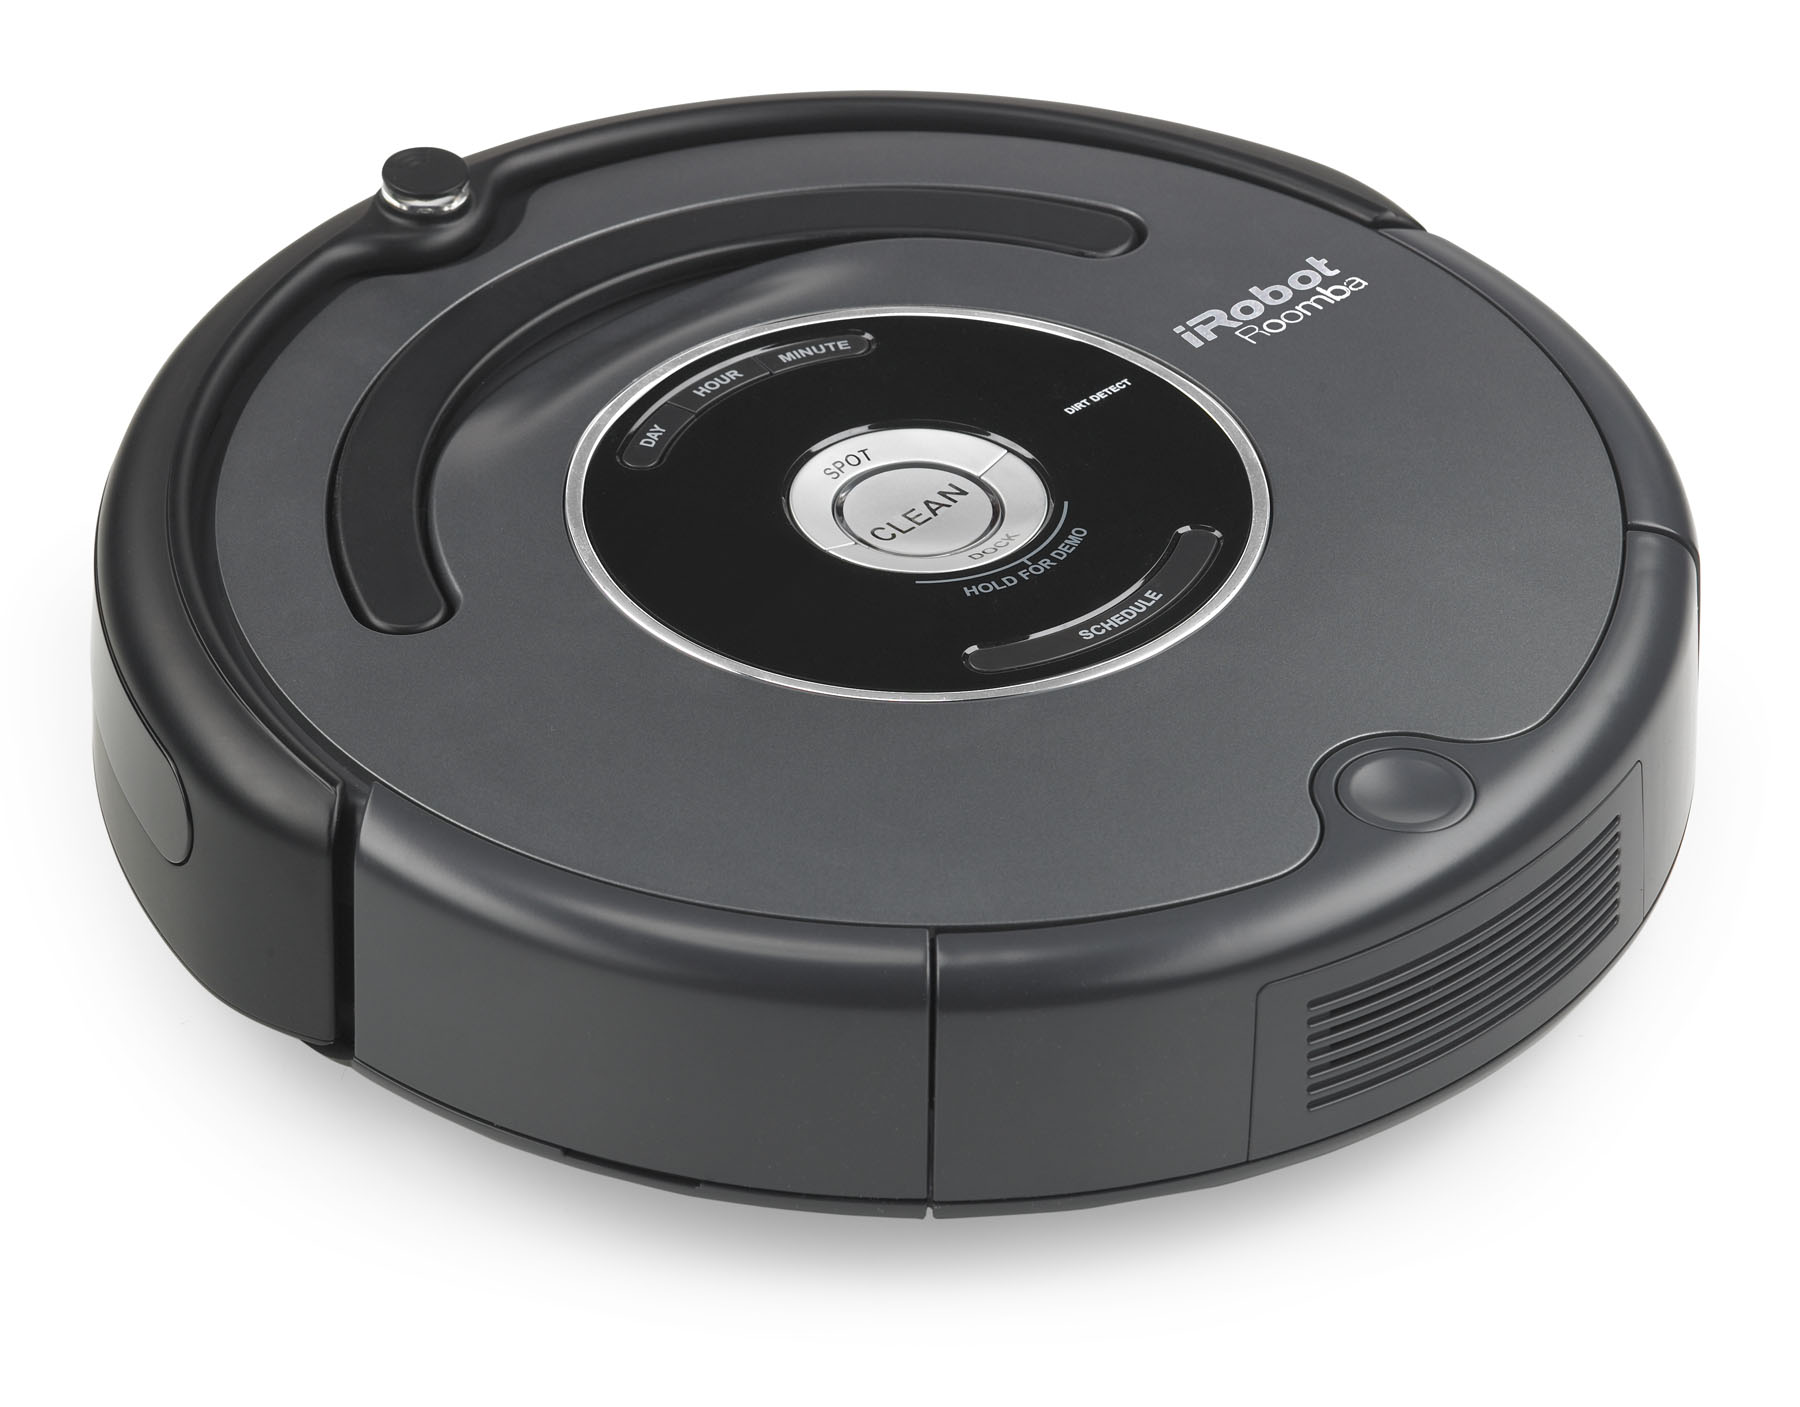
\includegraphics[height=90pt]{images/roomba560_sideview.jpg} 
%	\label{fig:Roomba}
%    \caption{Roomba cleaning robot}
%\end{figure}

%%%%%%%%%%%%%%%%%%%%%%%%%%%%%%%%%%%%%%%%%%%%%%%%%%%
%% Section Goal
\section{Goal}
\label{sec:Goal}
Our objective to design a swarm of autonomous mobile
systems that will be able to perform the following:

\begin{enumerate}
\item{ Identify the object to find (which will be presented by a human) }
\item{Two of the robots, seekers, search for an object in an indoor environment, which may
not be known beforehand but the object is within the robot reach }
\item{ The seekers move towards the object and signal a third robot that they have reached it(using
a sound signal such as a beep or some visual cue) }
\item{The third robot, confirmer, navigates towards the object}
\item{The confirmer has a better sensor suite than the seeker and tells if it is indeed the specific object}
\item{(Optionally) The robots should be able to come back to their 
initial position}
\end{enumerate}

%%%%%%%%%%%%%%%%%%%%%%%%%%%%%%%%%%%%%%%%%%%%%%%%%%%
%% Section Robot Platform
\section{Robot Platform}
Given the goal presented on Section \ref{sec:Goal}, 
our choice of platforms are: 

\begin{itemize}
\item{
A Turtlebot%(Fig.\ref{fig:Turtlebot1}),
%which combines a low-cost set of hardware as briefly explained below:
with the following sensor suite.

%------------------------------------------------------------
% Image: Turtlebot
%\begin{figure}[h]
%	\centering
%	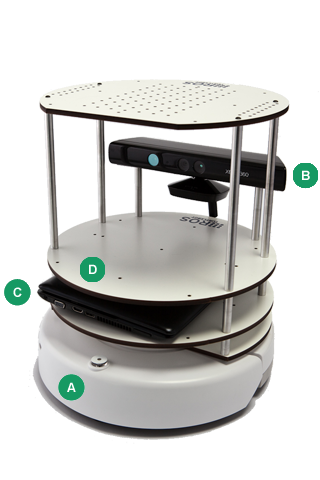
\includegraphics[height=120pt]{images/turtlebotlabels3.png} 
%	\label{fig:Turtlebot1}
%    \caption{Robot Platform: Turtlebot}
%\end{figure}

%\subsection*{Hardware}
%\begin{itemize}
%\item{Mobile platform: iRobot Create (similar to the Roomba)}
%\item{ASUS 1215N: Intel Atom D525 Dual Core Processor, 2GB RAM,
%NVidia Discrete Graphics Processor and 250GB of Hard Drive}
%\end{itemize}

%\subsection*{Sensor Suite}
\begin{itemize}
\item{150 degrees/second single Axis Gyro}
\item{Microsoft Kinect  for 3D Sensing capabilities}
\item{Left and Right bumpers (iCreate)}
\item{Left and Right wheels encoder(iCreate)}
\end{itemize}
}

\item{
 A pair of Amigobots% (Fig. \ref{fig:amigobot})
 %, which also combine a low-cost set of hardware as follow:
with the following sensor suite.

%\subsection*{Hardware}
%\begin{itemize}
%\item{Microcontroller: 44mhz Renesas SH2-7144 processor}
%\item{Wireless Ethernet-to-serial device}
%\item{Gyroscope Heading Correction device}
%\end{itemize}

%\subsection*{Sensor Suite}
\begin{itemize}
\item{A Microsoft Lifecam Studio1080p HD Webcam}
\item{8 sonars}
\item{2 position encoders}
\end{itemize}
}
\end{itemize}

%------------------------------------------------------------
%Image:Amigobot
%\begin{figure}[h]
%	\centering
%	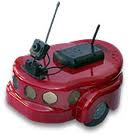
\includegraphics[height=90pt]{images/amigobot.jpg} 
%	\label{fig:amigobot}
%    \caption{Robot Platform: Amigobot}
%\end{figure}


%%%%%%%%%%%%%%%%%%%%%%%%%%%%%%%%%%%%%%%%%%%%%%%%%%%
%% Section Environment
\section{Environment}
\subsection*{Simulation}
For most of the development part of this project we intend to
use the player/stage/gazebo as our simulation software. Turtlebot and Amigobot are both part of its robot suite.
We will perform a simulation of our algorithms using the Gazebo 3D simulation environment.

\subsection*{Real hardware}
Our group currently has a Kinect, and we are arranging to borrow
a TurtleBot from one of the Labs at the Center for Robotics
and Intelligent Machines at Georgia Tech. And with enough time we will implement our algorithm onto real hardware. 
However, if this is not feasible, we should still be able to perform our experiments
purely in a virtual setup.

\end{document}




















